\documentclass[12pt,a4paper]{article}
\usepackage{amsmath,amssymb}
\usepackage{graphicx}
\usepackage{float}
\usepackage{tikz}
\usetikzlibrary{shapes, arrows, positioning}


\usepackage{amsmath,amssymb,mdframed}            % AMS package gives better equation layouts
\setcounter{page}{5}                    % sets first page number to 2
\setlength{\oddsidemargin}{-0.25in}     % set left margin
\setlength{\textwidth}{6.5in}           % set text width
\setlength{\topmargin}{-0.5in}          % controls layout at
\setlength{\headsep}{0.5in}             % top of page
\setlength{\textheight}{9.0in}          % set text length



\makeatletter
\renewcommand{\@oddhead}{\hfill MA3600/2014-2015-solution}  % sets header
\renewcommand{\@oddfoot}{\hfil \arabic{page} \hfil}    % sets page footer
\makeatother

\renewcommand{\labelenumi}{\arabic{enumi}} % Sets the first level of enumerate to be arabic (normal) numbers
\renewcommand{\labelenumii}{(\alph{enumii})} %Sets the second level of enumerate to be (a), (b), (c), .....
\renewcommand{\labelenumiii}{(\roman{enumiii})} % Sets the third level of enumerate to be (i), (ii), (iii), ....



\begin{document}
\null \vskip1cm
\begin{enumerate}
\setcounter{enumi}{3}

\renewcommand\labelenumi{\bfseries\theenumi.}

\item

    \begin{enumerate}
        \item Provide definitions for the following terms:
            \begin{itemize}
                \item Normal form game.\\


                A $N$ player \textbf{normal form game} consists of:
                \begin{itemize}
                \item A finite set of $N$ players;
                \item Strategy spaces for the players: $S_1, S_2, S_3, \dots S_N$;
                \item Payoff functions for the players: $u_i:S_{1}\times S_2\dots\times S_N\to \mathbb{R}$
                \end{itemize}

                ~\hfill{[1]}

                \item Strictly dominated strategy.\\

                In an $N$ player normal form game. A pure strategy $s_i\in S_i$ is said to be \textbf{strictly dominated} if there is a strategy $\sigma_i\in \Delta S_i$ such that $u_i(\sigma_i,s_{-i})>u_{i}(s_i,s_{-i})$ for all $s_{-i}\in S_{-i}$ of the other players.

                ~\hfill{[1]}

                \item Weakly dominated strategy.\\

                In an $N$ player normal form game. A pure strategy $s_i\in S_i$ is said to be \textbf{weakly dominated} if there is a strategy $\sigma_i\in \Delta S_i$ such that $u_i(\sigma_i,s_{-i})\geq u_{i}(s_i,s_{-i})$ for all $s_{-i}\in S_{-i}$ of the other players and there exists a strategy profile $\bar s\in S_{-i}$ such that $u_i(\sigma_i,\bar s)> u_{i}(s_i,s_{-i})$.

                ~\hfill{[1]}

                \item Best response strategy.\\

                In an $N$ player normal form game. A strategy $s^*$ for player $i$ is a best response to some strategy profile $s_{-i}$ if and only if $u_i(s^*,s_{-i})\geq u_{i}(s,s_{-i})$ for all $s\in S_i$.

                ~\hfill{[1]}

                \item Nash equilibrium.\\

                In an $N$ player normal form game. A Nash equilibrium is a strategy profile $\tau = (\tilde s_1,\tilde s_2,\dots,\tilde s_N)$ such that:

                $$u_i(\tilde s)\geq u_i(\bar s_i,\tilde s_{-i})\text{ for all }i$$
                ~\hfill{[1]}
            \end{itemize}

       \item
        Consider the following game:

            \[\begin{pmatrix}
            (7,3) & (0,2)\\
            (2,0) & (6,2)\\
            \end{pmatrix}\]

       \begin{enumerate}
        \item By clearly stating the techniques used: obtain all (if any) pure Nash equilibria.

            We attempt to identify best responses under the assumption of common knowledge of rationality:


            \[\begin{pmatrix}
                    (\underline{7},\underline{3}) & (0,2)\\
                    (2,0) & (\underline{6},\underline{2})\\
            \end{pmatrix}\]

            There are two pure nash equilibria: \(\{(r_1, c_1), (r_2,c_2)\}\).

        ~\hfill{[4]}

        \item Sketch the utilities to player 1 (the row player) assuming that the 2nd player (the column player) plays a mixed strategy: $\sigma_2 = (y,1-y)$.

        We have:

        $$u_1(r_1,\sigma_2)=7y$$

        and

        $$u_1(r_2,\sigma_2)=2y+6(1-y)=6-4y$$

        ~\hfill{[1]}

        Which gives:

        \begin{center}
            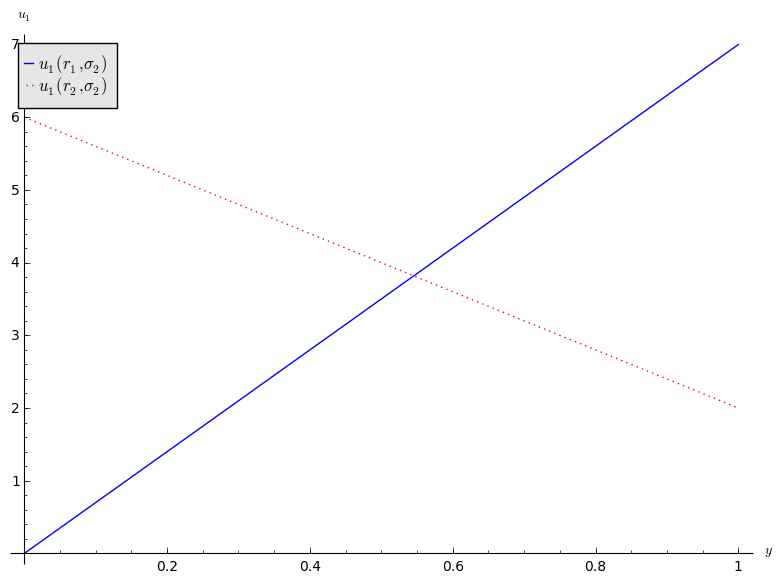
\includegraphics[width=.5\textwidth]{./plots/2014-2015-plt01.png}
        \end{center}

        ~\hfill{[1]}

        \item Sketch the utilities to player 2 (the column player) assuming that the 1st player (the row player) plays a mixed strategy: $\sigma_1 = (x,1-x)$.

        We have:

        $$u_2(\sigma_1,s_1)=3x$$

        and

        $$u_2(\sigma_1,s_2)=2$$

        ~\hfill{[1]}

        Which gives:

        \begin{center}
            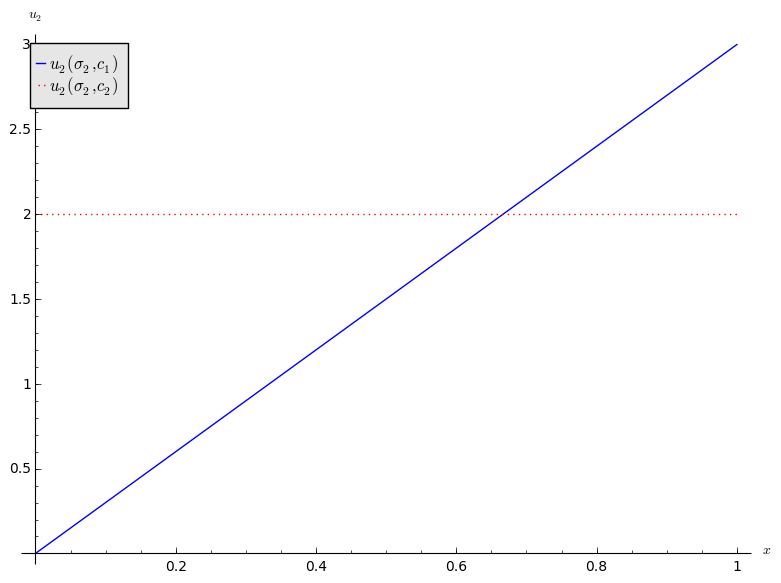
\includegraphics[width=.5\textwidth]{./plots/2014-2015-plt02.png}
        \end{center}

        ~\hfill{[1]}

        \item State, prove and use the Equality of Payoffs theorem to obtain all Nash equilibria for
            the game.

            The equality of payoffs theorem states:

            In an $N$ player normal form game if the strategy profile $(\sigma_i,s_{-i})$ is a Nash equilibria then:

            $$u_{i}(\sigma_i,s_{-i})=u_{i}(s,s_{-i})\text{ for all }s\in\mathcal{S}(\sigma_i)\text{ for all }1\leq i\leq N$$

            ~\hfill{[1]}

            \textbf{Proof:}

            If $|\mathcal{S}(\sigma_i)|=1$ then the proof is trivial.

            We assume that $|\mathcal{S}(\sigma_i)|>1$. Let us assume that the theorem is not true so that there exists $\bar s\in\mathcal{S}(\sigma)$ such that

            $$u_{i}(\sigma_i,s_{-i})\ne u_{i}(\bar s,s_{-i})$$

            Without loss of generality let us assume that:

            $$\bar s=\text{argmax}_{s\in\mathcal{S}(\sigma)}u_i(s,s_{-i})$$

            Thus we have:

            $$\begin{aligned}
            u_i(\sigma_i,s_{-i})&=\sum_{s\in\mathcal{S}(\sigma_i)}\sigma_i(s)u(s,s_{-i})\\
            &\leq \sum_{s\in\mathcal{S}(\sigma_i)}\sigma_i(s)u(\bar s,s_{-i})\\
            &\leq u(\bar s,s_{-i})\sum_{s\in\mathcal{S}(\sigma_i)}\sigma_i(s)\\
            &\leq u(\bar s,s_{-i})\\
            \end{aligned}$$

            Giving:

            $$u_{i}(\sigma_i,s_{-i})< u_{i}(\bar s,s_{-i})$$

            which implies that $(\sigma_i,s_{-i})$ is not a Nash equilibrium.

            ~\hfill{[4]}

            To obtain the mixed Nash equilibrium missing from the two pure Nash equilibria already found:

            $$u_1(r_1,\sigma_2)=u_1(r_2,\sigma_2)\Rightarrow \tilde y=6/11$$
            $$u_2(\sigma_1, c_1)=u_2(\sigma_1, c_2)\Rightarrow \tilde x=2/3$$

            Thus, all the Nash equilibria are given by:

            \[\{((1,0),(1,0)),((0,1),(0,1)),((2/3,1/3),(6/11,5/11))\}\].

            ~\hfill{[1]}

        \item Consider the same game with an extra strategy for the row player:

            \[\begin{pmatrix}
            (7,3) & (0,2)\\
            (3,1) & (3,1)\\
            (2,0) & (6,2)\\
            \end{pmatrix}\]

            By directly calculating the set of best response strategies \(B_1\) for the row player obtain all Nash equilibrium for this new game.
            State any theorem(s) used.

            Here is the plot of the best utilities of player one with the new strategy:

            \begin{center}
                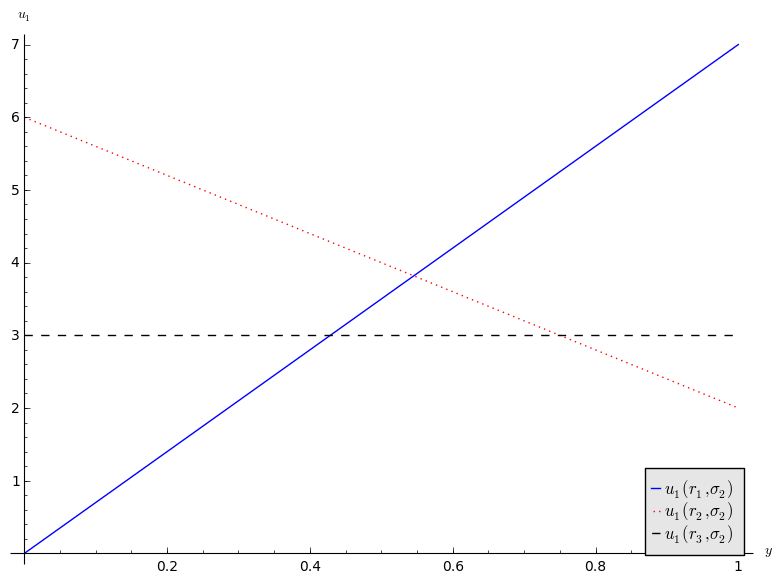
\includegraphics[width=.5\textwidth]{./plots/2014-2015-plt03.png}
            \end{center}

            ~\hfill{[3]}

            We see that \(B_1=\{r_1,r_2\}\), however by the theorem stating the equality of best response strategies to sets of undominated strategies in two player games we know that the Nash equilibria are the same:

            \[\{((1,0),(1,0)),((0,1),(0,1)),((2/3,1/3),(6/11,5/11))\}\].

            ~\hfill{[3]}

    \end{enumerate}
    \end{enumerate}

\newpage
\item

    This question considers evolutionary population games.
    Throughout the following game is considered:

    Road users in a given country can choose to drive on either the left (\(L\)) side or the right (\(R\)) side of the road.
    The strategy set in this game is \(S=\{L, R\}\).

    If all users drive on the same side of the road then no accidents will occur.
    If users drive on the opposite side and meet each other then they may have an accident.

    Considering a population vertor \(\chi=(x,1-x)\) where \(x\) is the proportion of the population using strategy \(L\), the utilities are given by:

    \[u(L,\chi)=1+x\]
    and
    \[u(R,\chi)=1+(1-x)\]


    \begin{enumerate}

            \item Define a stable strategy in a population game.

                If we consider \(\chi\) to be the startegy profile where all members of the population play \(\sigma^*\) then a population will be stable if:

                $$\sigma^*\in\text{argmax}_{\sigma\in\Delta S}u(\sigma,\chi)$$

                \hfill{[2]}

            \item State and prove a theorem giving a necessary condition for stable strategies.
                Use this theorem to obtain all potential evolutionary stable strategies in the above situation.


        In a population game, consider \(\sigma^*\in\Delta S\) and the population profile \(\chi\) generated by \(\sigma^*\). If the population is stable then:

        $$u(s,\chi)=u(\sigma^*,\chi)\text{ for all }s\in\mathcal{S}(\sigma^*)$$

                \hfill{[1]}

        (Recall that \(\mathcal{S}(s)\) denotes the support of \(s\).)

        Proof:

        If \(|\mathcal{S}(\sigma^*)|=1\) then the proof is trivial.

        We assume that \(|\mathcal{S}(\sigma^*)|>1\). Let us assume that the theorem is not true so that there exists \(\bar s\in\mathcal{S}(\sigma^*)\) such that:

        $$u(\sigma^*,\chi)\ne u(\bar s,\chi)$$

        Without loss of generality let us assume that:

        $$\bar s=\text{argmax}_{s\in\mathcal{S}(\sigma^*)}u(s,\chi)$$

        Thus we have:

        $$\begin{aligned}
        u_{i}(\sigma^*,\chi)&=\sum_{s\in\mathcal{S}(\sigma^*)}\sigma^*(s)u(s,\chi)\\
        &\leq\sum_{s\in\mathcal{S}(\sigma^*)}\sigma^*(s)u(\bar s,\chi) \\
        &\leq u(\bar s,\chi)\sum_{s\in\mathcal{S}(\sigma^*)}\sigma^*(s) \\
        &\leq u(\bar s,\chi)
        \end{aligned}$$

        Which gives:

        $$u(\sigma^*,\chi)< u(\bar s,\chi)$$

        which implies that the population is not stable.

                \hfill{[4]}

        Using this we have the 3 potential strategies:

        \begin{itemize}
            \item $\sigma_L=(1,0)$
            \item $\sigma_R=(0,1)$
            \item $\sigma_M=(x,1-x)$ where (using the stated result): $1+x=x+(1-x)\Rightarrow x=1/2$.
        \end{itemize}

            \hfill[1]

            \item Define a post entry population.

                Consider a population where all individuals initially play \(\sigma^*\).
                If we assume that a small proportion \(\epsilon\) start playing \(\sigma\).
                The new population is called the post entry population and will be denoted by \(\chi_{\epsilon}\).

                \hfill{[2]}

            \item Define an evolutionary stable strategy.

                A strategy \(\sigma^*\in\Delta S\) is called an Evolutionary Stable Strategy if there exists an \(0<\bar\epsilon<1\) such that for every \(0<\epsilon<\bar \epsilon\) and every \(\sigma\ne \sigma^*\):

                $$u(\sigma^*,\chi_\epsilon)>u(\sigma,\chi_\epsilon)$$

                \hfill{[2]}

            \item Obtain all evolutionary stable strategies for the described game.

                \[\chi_{\epsilon}=\sigma^*+\epsilon(\sigma^*-\sigma)\]

                and

                \[\delta=(\mu-\mu^*)(u(L,\chi_{\epsilon}) - u(R, \chi_{\epsilon}))\]

                \hfill{[3]}

                we have:

                \[u(L,\chi_{\epsilon})=1+x_{\epsilon}=1+\mu^*+\epsilon(\mu-\mu^*)\]
                \[u(R,\chi_{\epsilon})=2-x_{\epsilon}=2-\mu^*-\epsilon(\mu-\mu^*)\]

                thus:

                \[\delta=(\mu-\mu^*)(-1+2\mu^*+2\epsilon(\mu-\mu^*))\]

                \hfill{[3]}

                Considering each case:

                \begin{itemize}
                    \item \(\mu^*=1\):

                        \[\delta=(1-\mu)(1+2\epsilon(\mu-1))\]

                        \(\epsilon < 1/2\) implies that \(\delta>0\) as required: so ESS.

                \hfill{[2]}

                    \item \(\mu^*=0\):

                        \[\delta=(-\mu)(-1+2\epsilon\mu)\]

                        \(\epsilon < 1/2\) implies that \(\delta>0\) as required: so ESS.

                \hfill{[2]}

                    \item \(\mu^*=1/2\):

                        \[\delta=(1/2-\mu)(2\epsilon(\mu-1/2))\]
                        \[\delta=(1/2-\mu)^2(-2\epsilon)\]

                        Thus \(\delta<0\) for all \(\epsilon\): not an ESS.

                \hfill{[2]}

                \end{itemize}

            \item Offer an interpretation for the answer to question (e).

                We see that there are 2 stable situations: a social convention in which everyone drives on the same side of the road.
                1 potential situation however (everyone picking a side randomly) is not stable.
                \hfill{[1]}
    \end{enumerate}

\newpage
\item


    \begin{enumerate}

        \item Define a characteristic function game \(G=(N,v)\).

        A characteristic function game \(G\) is given by a pair \((N,v)\) where \(N\) is the number of players and \(v:2^{[N]}\to\mathbb{R}\) is a characteristic function which maps every coalition of players to a payoff.

        \hfill{[2]}

        \item Define the Shapley value.

        Given \(G=(N,v)\) the Shapley value of player \(i\) is denoted by \(\phi_i(G)\) and given by:

        $$\phi_i(G)=\frac{1}{N!}\sum_{\pi\in\Pi_n}\Delta_\pi^G(i)$$

        \hfill{[2]}

        \item Obtain the Shapley value for the following characteristic function games:

            \[
                v_1(c) = \begin{cases}
                    6,& \text{if }c=\{1\}\\
                    6,& \text{if } c=\{2\}\\
                    7,& \text{if } c=\{3\}\\
                    7,& \text{if } c=\{1,2\}\\
                    7,& \text{if } c=\{2,3\}\\
                    20,& \text{if } c=\{1,3\}\\
                    40,& \text{if } c=\{1,2,3\}\\
                \end{cases}
            \]

            Applying the formula, the shapley value is: \((46/3, 53/6, 95/6)\).
            \hfill{[4]}

            \[
                v_2(c) = \begin{cases}
                    100,& \text{if }c=\{1\}\\
                    6,& \text{if } c=\{2\}\\
                    7,& \text{if } c=\{3\}\\
                    100,& \text{if } c=\{1,2\}\\
                    7,& \text{if } c=\{2,3\}\\
                    100,& \text{if } c=\{1,3\}\\
                    100,& \text{if } c=\{1,2,3\}\\
                \end{cases}
            \]

            Applying the formula, the shapley value is: \((191/2,2,5/2)\).
            \hfill{[4]}

        \item  For a given charachteristic function game \(G=(N,v)\) a payoff vector \(\lambda\) is efficient if:

            \[\sum_{i=1}^{N}\lambda_i=v(\Omega)\]

            Prove that the Shapley value is efficient.

            \begin{align}
                \sum_{i=1}^{N}\Delta_{\pi}^{G}(i)=&v(S_{\pi}(1)\cup \{1\})-v(S_{\pi}(1))+v(S_{\pi}(2)\cup \{2\})-v(S_{\pi}(2))\dots v(S_{\pi}(N)\cup N)-v(S_{\pi}(N))\nonumber\\
                =&v(S_{\pi}(N)\cup N)=v(N)\nonumber
            \end{align}

        \hfill{[4]}

            taking the mean over all permutations (which is by definition the Shapley value) we have the required result.

        \hfill{[2]}

        \item For \(G(N,v)\) a payoff vector \(\lambda\) is symmetric the following holds:

        If \(v(C\cup i)=v(C\cup j)\) for all \(C\in 2^{\Omega}\setminus\{i,j\}\) then \(x_i=x_j\).

        Prove that the Shapley value is symmetric.

        Assume that \(i\) and \(j\) are symmetric. Given a permutation \(\pi\), let \(\pi'\) denote the permutation obtained by swapping \(i\) and \(j\).

        - Assume that \(i\) precedes \(j\) in \(\pi\), this gives \(S\_{\pi}(i)=S\_{\pi'}(j)\), if we let \(C=S_{\pi'}(j)\):

            $$\Delta_{\pi}^{G}(i)=v(C\cup \{i\})-v(C)$$

            and

            $$\Delta_{\pi'}^{G}(j)=v(C\cup \{j\})-v(C)$$

        \hfill{[2]}

            By symmetry \(\Delta\_{\pi}^{G}(i)=\Delta\_{\pi'}^{G}(j)\).

        \hfill{[1]}

        - Assume that \(i\) does not precede \(j\) in \(\pi\), let \(C=S_{\pi}(i)\setminus \{j\}\). We have:

            $$\Delta_{\pi}^{G}(i)=v(C\cup \{i\} \cup \{j\})-v(C\cup \{j\})$$

            and

            $$\Delta_{\pi'}^{G}(j)=v(C\cup \{j\} \cup \{i\})-v(C\cup \{i\})$$

        \hfill{[2]}

            Since \(C\subseteq N\) and \(i,j\notin C\) we have by symmetry \(v(C\cup\{i\})=v(C\cup\{j\})\) and therefore \(\Delta\_{\pi}^{G}(i)=\Delta\_{\pi'}^{G}(j)\).

        We have that \(\Delta_{\pi}^{G}(i)=\Delta_{\pi'}^{G}(j)\) for all \(\pi\in\Pi_N\), there is an abvious bijection between all \(\pi\) and corresponding \(\pi'\) thus:

        $$\phi_i(G)=1/n!\sum_{\pi\in\Pi_N}\Delta_{\pi}^{G}(i)=\sum_{\pi\in\Pi_N}\Delta_{\pi'}^{G}(j)=\phi_j(G)$$

        as required.

        \hfill{[2]}


    \end{enumerate}
\end{enumerate}


\makeatletter
\renewcommand{\@oddfoot}{\hfil \arabic{page}X \hfil}    % sets last page footer
\makeatother

\end{document}
